\documentclass{article}
\usepackage[utf8]{inputenc}
\usepackage{setspace}
\usepackage{hyperref}
\usepackage{url}
\usepackage[T2A]{fontenc}	
\usepackage{ dsfont }
\usepackage{amssymb}
\usepackage[english, russian]{babel}
\usepackage{graphicx}
\usepackage{amsmath}
\usepackage{tikz}
\usetikzlibrary{matrix}
%\DeclareGraphicsExtensions{.pdf,.png,.jpg}
\usepackage{float}
\usepackage{natbib}
\usepackage{algorithmic}
\usepackage[ruled,vlined]{algorithm2e}
\title{Choosing agreed models for building a neural interface}
\author{Kulakov Yaroslav}
\date{February 2021}
\doublespacing

\newcommand{\argmin}{\mathop{\arg \min}\limits}
\newcommand{\argmax}{\mathop{\arg \max}\limits}

\begin{document}

\maketitle




\section{Annotation}
The work solves the problem of building a neurocomputer interface. It is required to predict the three-dimensional trajectory of limb movement based on signals from the cerebral cortex. The complexity of the problem lies in the fact that the description of the original signals is redundant and highly correlated. It is proposed to apply methods of reducing the dimensionality of the original space with matching models in the hidden space. To solve the problem, linear and nonlinear agreement models are used. The target and latent spaces obtained by a pair of models are analyzed. Experimental results confirm that the proposed method improves the quality of model predictions.

\section{Introduction}
Neurocomputer interfaces (BCI) decode brain activity, make it possible to process it with machine learning models in order to predict actions by extracting useful information from the data obtained and presenting it in a human-interpretable form \cite{general_purpose_1300799} \cite{BLANKERTZ20101303}. The descriptions of the EEG and EEC data are high-dimensional due to the high complexity of the brain and the large amount of information at each point in time. The signals are highly correlated time series. To obtain uncorrelated and informative features, the problem of reducing the dimension of the original space is solved.\cite{feature_selection_ecog} \cite{ATYABI2013319} \cite{7330455} \par

The article \cite{qpfs} compares feature selection algorithms. The Quadratic Programming Feature Selection \cite{qpfs} algorithm is considered in comparison withс LARS \cite{MICHE20112413}, Lasso \cite{zhao2007stagewise}, Ridge \cite{ridge} and feature selection with the genetic algorithm \cite{tan2008genetic}. \par
A comparison is made with the methods PLS, PCA\cite{abdi2003pls} \cite{wegelin2000survey}, other nonlinear models. When solving the problem of feature selection, two functionalities are simultaneously optimized: the correlation between features is minimized and the information content of features in relation to the target is maximized. The task is complicated by the fact that features and targets are of different nature. Therefore, different models are built for different spaces, and the final model is obtained by matching the base ones.

\par
In this paper, linear and nonlinear signal decoding models are investigated. The quality, stability and complexity of the models under consideration are assessed. \par
In this paper, we propose a robust algorithm for decoding the brain activity signal. The proposed algorithm consists of the following stages:
\begin{itemize}
    \item construction of a latent space of a lower dimension, with a minimum correlation of features with each other and a maximum correlation of features with a predicted signal;
    \item building a predictive model in the resulting space;
\end{itemize}

\section{Problem statement}

The sample is considered $(\mathbf{X}, \mathbf{Y}).$ $ \mathbf{X} \in \mathbb{R}^{m \times n},\mathbf{Y} \in \mathbb{R}^{m \times r}$, where $\mathbf{X}$ --- time series of electrocorticogram, $\mathbf{Y}$ --- time series of hand position in 3D space. Here $m$ --- number of timestamps, $n$ --- the number of electrodes used to pick up the signal, $r = 3$ --- the number of coordinates in three-dimensional space. The data contains records of the trajectory of the hand movement in 3D space and the ECoG signal. It is required to build a pair of agreed models predicting the path of the brush$Y_{t+1}$, according to the series $X_0 \dots X_{t+1}$ and $Y_0 \dots Y_t$, where $\mathbf{X_t}, \mathbf{Y_t}$ --- multidimensional feature descriptions of brain activity and coordinates at a moment in time $t$.
\subsection{Regression in the original data space}
Consider a family of models $f: \mathbf{X} \rightarrow \mathbf{Y}$, where $\mathbf{X} \in \mathbb{R}^{m \times np}$ --- the obtained time series of features after the wavelet transformation, and $\mathbf{Y} \in \mathbb{R}^{m \times r}$ --- a series of brush paths. Here $p$ --- the number of features obtained for each time point and each electrode by the wavelet transform. The problem is to find the model $f^*$, that minimizes the given error functional $\mathcal{L}$.
\begin{equation}\label{eq1} 
	f^* = \argmin_f \mathcal{L}(f, \mathbf{X}, \mathbf{Y}).
\end{equation}
We will consider a parametric family of models $f(x, \theta)$, where $\mathbf{\theta}$ --- model parameters. Then the problem of finding a model $f^*$ is equivalent to the problem of finding parameters $\mathbf{\theta^*}$:
\begin{equation}\label{eq2} 
\theta^* = \argmin_{\theta} \mathcal{L}(\theta, X, Y).
\end{equation}
The linear regression model is considered as a basic model:
$f(\mathbf{X}, \mathbf{\theta}) = \mathbf{\theta}^T\mathbf{X}$.
\subsection{Regression in the target signal space}
Regression models of time series are considered $f : \mathbf{Y} \rightarrow \mathbf{Y}$. Where $\mathbf{Y} \in  \mathbb{R}^{m \times r}$ For each coordinate, consider the time series $\{y_t\}$. The problem is posed of finding a model $f^*$, that predicts from the last $y_{t^{'}-p} \dots y_{t^{'}}$ the value $y_{t^{'}+1}$ for all $t^{'} \in \{0, \dots t\}$, minimizing some error functional $ \mathcal{L}$.
\begin{equation}\label{eq3} 
	f^* = \argmin_f \mathcal{L}(f, \mathbf{Y}).
\end{equation}

Similarly, the problem of finding a model $f^*$ is equivalent to the problem of finding parameters $\theta^*$.
\begin{equation}\label{eq4} 
\theta^* = \argmin_{\theta} \mathcal{L}(\theta, \mathbf{Y}).
\end{equation}
Autoregressive model is used as basic predictive models $AR$, as well as modify it ($ARIMAX$ \cite{7514029} and etc).
\subsection{The problem of high dimensionality and correlation}
The high dimension of the space $ X $ and the linear dependence of the columns leads to data redundancy and instability of models. Therefore, the problem is posed of finding the functions $\phi: X^n \rightarrow T^l$ и  $Y^r \rightarrow U^s$, representing the original spaces $X, Y$ in hidden spaces of lesser dimension $T, U$ $(l < n, s < r)$, maximizing the covariance between the independent and target variables in these spaces. The resulting matrices are matrices of hidden representations in the latent space.

\textbf{Definition}. Let's call the space $\mathbb{T} \subset \mathbb{R}^{l}$ a hidden space for space $\mathbb{X} \in \mathbb{R}^{n}(l \leqslant n),$ if there is a function $\varphi_{e}: \mathbb{X} \rightarrow \mathbb{T}$ and function $\varphi_{d}: \mathbb{T} \rightarrow \mathbb{X}$ such that
$$
\mathbf{x} \in \mathbb{X} \quad \exists \mathbf{t} \in \mathbb{T}: \varphi_{d}\left(\varphi_{e}(\mathbf{x})\right)=\varphi_{d}(\mathbf{t})=\mathbf{x}
$$
Function $\varphi_{e}(\mathbf{x})$ called the object encoding function $\mathbf{x},$ function $\varphi_{d}(\mathbf{t})$
called the decoding function.

Similarly, we introduce the definition of the hidden space $\mathbb{U} \subset \mathbb{R}^{s}$ for the target space  $\mathbb{Y}$, encoding functions $\psi_{e}: \mathbb{Y} \rightarrow \mathbb{U}$ and decoding
$\psi_{d}: \mathbb{U} \rightarrow \mathbb{Y}$
$$
\mathbf{y} \in \mathbb{Y} \quad \exists \mathbf{u} \in \mathbb{U}: \psi_{d}\left(\psi_{e}(\mathbf{y})\right)=\psi_{d}(\mathbf{u})=\mathbf{y}
$$

The general scheme of the decoding problem takes the form of the following commutative diagrams:
\begin{equation}
		\begin{tikzpicture}
			\matrix (m) [matrix of math nodes,row sep=3em,column sep=4em,minimum width=2em]
			{
				\mathbb{X} \subset \mathbb{R}^n & \mathbb{Y} \subset \mathbb{R}^r \\
				\mathbb{T} \subset \mathbb{R}^l & \mathbb{U} \subset \mathbb{R}^s \\};
			\path[-stealth]
			(m-1-1) edge node [above] {$f$} (m-1-2)
			(m-2-1) edge [bend right=10] node [right] {$\varphi_d$} (m-1-1)
			(m-2-2) edge [bend left=10] node [left] {$\psi_d$} (m-1-2)
			(m-1-1) edge [bend right=10] node [left] {$\varphi_e$} (m-2-1)
			(m-1-2) edge [bend left=10] node [right] {$\psi_e$} (m-2-2)
			(m-2-1) edge node [above] {$h$} (m-2-2);
		\end{tikzpicture}
	\end{equation}

Model $PLS$ is used to construct the latent space.
\subsection{Model agreement}
\textbf{Definition}. Model matching is a method of combining models that predict a target variable across different spaces.
Weighted summation is used as a way to match the predictions of the two models. There are two predictions of the coordinate at a time  $t+1$ --- $\hat{y}_{PLS, t+1}[\ref{eq2}], \hat{y}_{AR, t+1}[\ref{eq4}]$. The final prediction will be the weighted sum of these predictions.\[\hat{y}_{t+1} = \alpha \times \hat{y}_{PLS, t+1} + (1 - \alpha) \times \hat{y}_{AR, t+1}.\] Где $\alpha$ --- the hyperparameter of the supermodel is fitted over the grid, minimizing the error functional.
\subsection{Metrics}
Let $ y $ be the test segment of a multidimensional time series of coordinates, and $ \hat {y} $ be the predicted one.  $y, \hat{y} \in \mathbb{R}^{m' \times r}$, where $m'$ --- segment length. The following external quality criteria were selected in the work:
\begin{itemize}
    \item $MSE(||y-\hat y||_2^2 )$ --- \text{Root mean square error}.
    \item $MAE(||y-\hat y||_1)$--- \text{Mean absolute error}.
    
\end{itemize}


\section{Theory}
\subsection{PLS}
The pseudocode of the PLS regression method is given in Algorithm \ref{alg1}.
The algorithm iteratively calculates one column $t_k$, $u_k$, $p_k$, $q_k$ at each of the $ l $ steps from  matrices $\mathbf{T}$, $\mathbf{U}$, $\mathbf{P}$, $\mathbf{Q}$ respectively. 
After calculating the next set of vectors, the next peer-to-peer approximations are subtracted from the matrices $ X $, $ Y $.
It is assumed that the original matrices ~$X$ and ~$Y$ are normalized (have zero mean and unit mean deviation).

\begin{algorithm}[h]\label{alg1}
	\caption{Algorithm PLS}
	\label{ch1:pls_pseudocode}
	\begin{algorithmic}[1]
		\REQUIRE $\mathbf{X}, \mathbf{Y}, l$;
		\ENSURE $\mathbf{T}, \mathbf{P}, \mathbf{Q}$;
    		\STATE normalize matrices $X$ and $Y$ by columns
		\STATE initialize $u_0$ (first column of matrix $\mathbf{Y}$)
		\STATE $\mathbf{X}_1 = \mathbf{X}; \mathbf{Y}_1 = \mathbf{Y}$
		\FOR{$k=1,\dots, l$}
		\REPEAT
		\vspace{0.1cm}
		\STATE $w_k := \mathbf{X}_k^{T} u_{k-1} / (u_{k-1}^{T} u_{k-1}); \quad w_k: = \frac{w_k}{\| w_k \|}$
		\vspace{0.1cm}
		\STATE $t_k := \mathbf{X}_k w_k$
		\vspace{0.1cm}
		\STATE $c_k := \mathbf{Y}_k^{T} t_k / (t_k^{T} t_k); \quad c_k: = \frac{c_k}{\| c_k \|}$
		\vspace{0.1cm}
		\STATE $u_k := \mathbf{Y}_k c_k$
		\UNTIL{$t_k$ does not stabilize}
		\vspace{0.1cm}
		\STATE $p_k:= \mathbf{X}_k^{T}t_k/(t_k^{T}t_k),\ 
		q_k := \mathbf{Y}_k^{T}t_k/(t_k^{T}t_k)$
		\vspace{0.2cm}
		\STATE $\mathbf{X}_{k+1} :=  X_k - t_k p_k^{T}$
		\vspace{0.2cm}
		\STATE $\mathbf{Y}_{k + 1} :=  Y_k - t_k q_k^{T}$ 
		\ENDFOR
	\end{algorithmic}
\end{algorithm}
\subsection{AR, SARIMAX}

The series $\{y_t\}$ is given. Let's fix the parameter $p$ --- the number of the last values of the series by which the next prediction will be built. For each value $y_t^{'}$ from the training part of the series, select the $ p $ preceding it. According to the resulting matrix$X^{m, p}$ train linear regression $X\theta = Y$, minimizing the functionality $MSE$.

\par
SARIMAX  \cite{7514029} extends the basic autoregressive model, takes into account the linear dependence on the past values of the series and on the errors of past predictions, and takes into account the seasonality.
 

\section{Experiment}
ECoG signal was taken from 64x electrodes, 1 kHz frequency. To form the feature tensor, each ECoG epoch was mapped to the time-frequency-spatial space using a wavelet transform  \cite{eliseyev2016penalized}, \cite{chao2010long}.The purpose of the experiment is to analyze the proposed matching procedure.
\subsection{Dataset description}
The dataset [compiled by A. Motrenko] consists of 20 records of two monkeys trying to reach a piece of food with their right hand. The data transformed using the wavelet transform is a tensor $X \in \mathds{R}^{T \times K \times W+1}$, where $W$ --- dimension for wave conversion coefficients. In addition, the original time series matrix for each sensor is added to the data. $Y$ remains unchanged. The data were prepared by Anastasia Motrenko and have already been divided into training and test samples. The training sample has the following dimensions:  $X:(12801, 32, 27)$, where $T = 12801$ --- number of timestamps, $K = 32$ --- number of electrodes, $W = 26$ --- the number of frequencies for constructing the conversion factors and one more value corresponding to the voltage on the sensor at a fixed point in time and the number of the sensor. $Y:(12801, 3)$, accordingly, there are three hand position coordinates for each timestamp.
\begin{figure}[H]
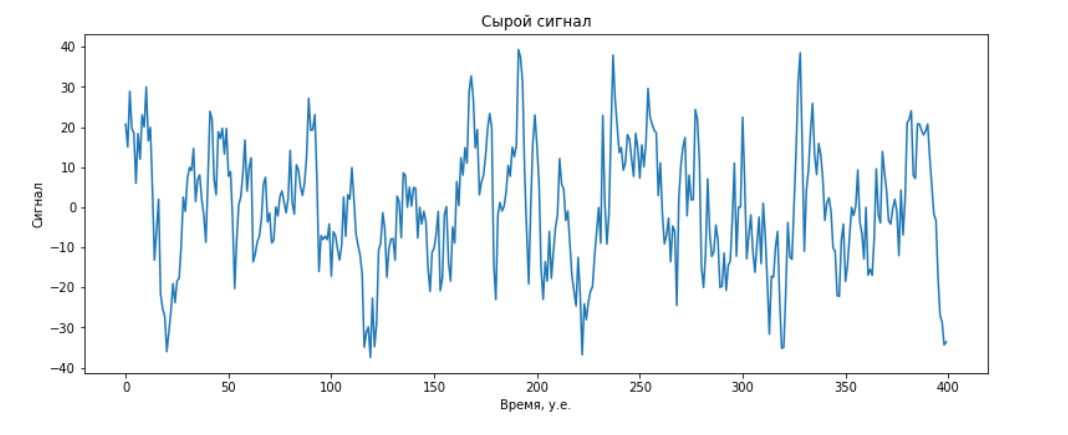
\includegraphics[scale=0.5]{images/8.png}
\end{figure}
Fig. 0. Visualization of the ECoG signal through one of the channels.
\subsection{Model analysis}
Using the grid, select the optimal dimension of the latent space for the PLS algorithm. Train PLS, AR, SARIMAX, LR models. Loop through the alpha parameter for agreement. Compare results.
\subsection{Performance}
After generating features and applying the PLS algorithm on the training data, the following predictions are obtained:

\begin{figure}[H]
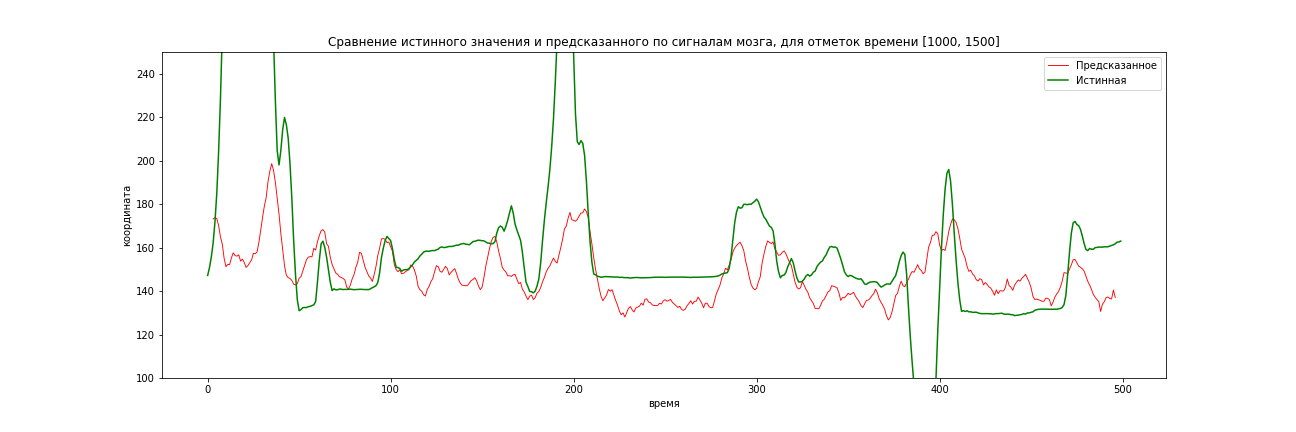
\includegraphics[scale=0.34]{images/1.png}
\end{figure}
Fig. 1. Coordinate prediction by PLS model from time series of brain activity $\mathbf{X}$
\begin{figure}[H]
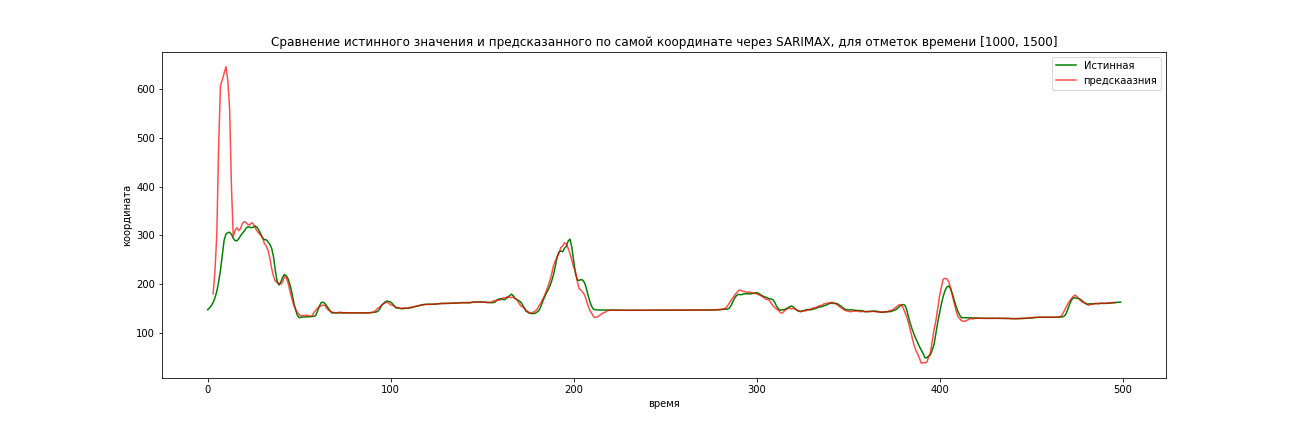
\includegraphics[scale=0.34]{images/2.png}
\end{figure}
Fig. 2. Coordinate prediction by SARIMAX model.
\begin{figure}[H]
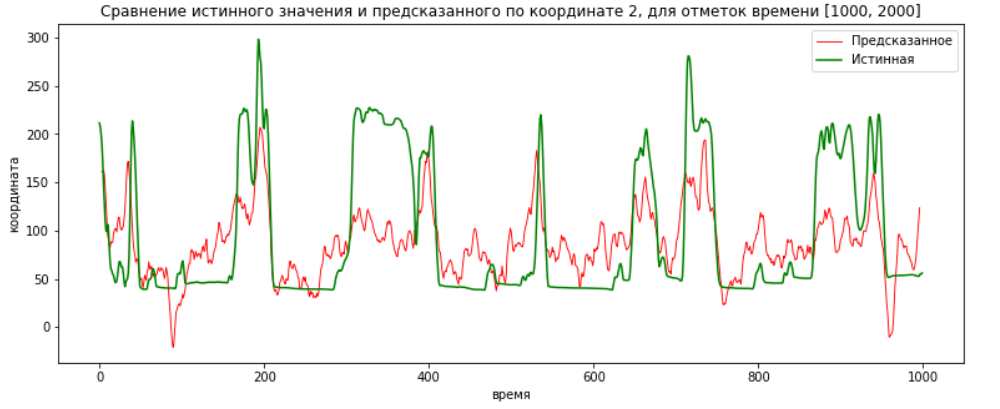
\includegraphics[scale=0.34]{images/3.png}
\end{figure}
Fig. 3. Result of model agreement, $\alpha = 0.86$.
\begin{figure}[H]
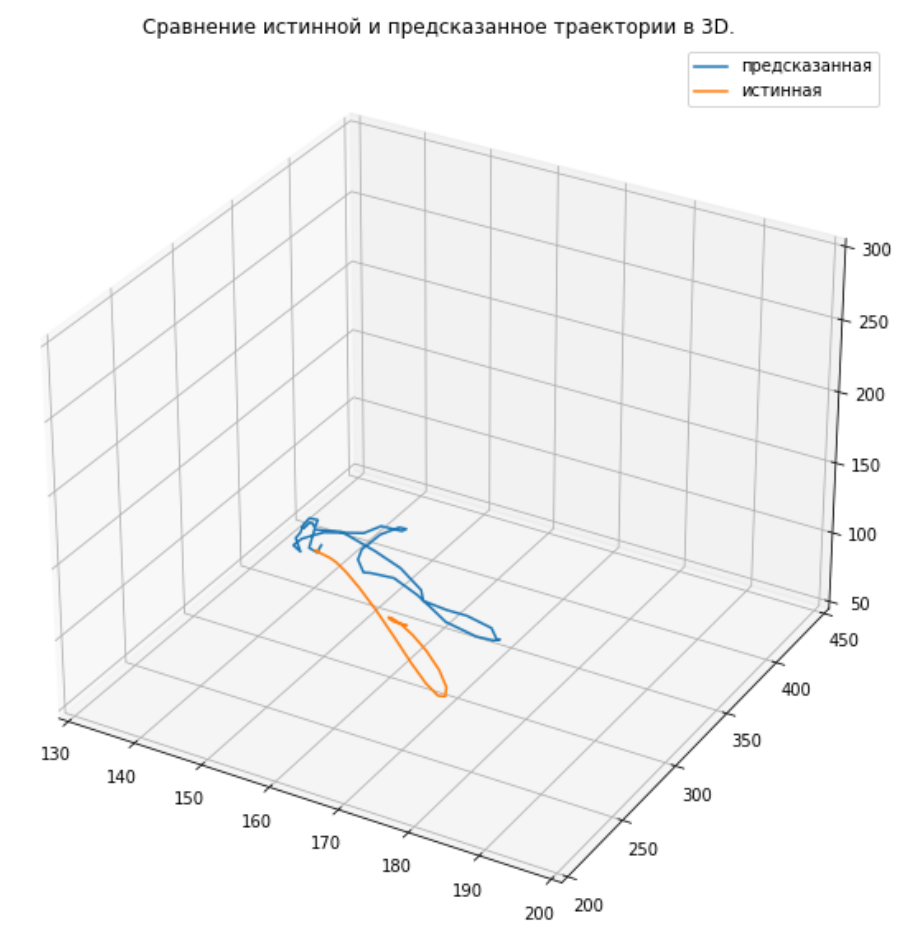
\includegraphics[scale=0.34]{images/4.png}
\end{figure}
Fig. 4. Coordinate prediction by AR model.
\begin{figure}[H]
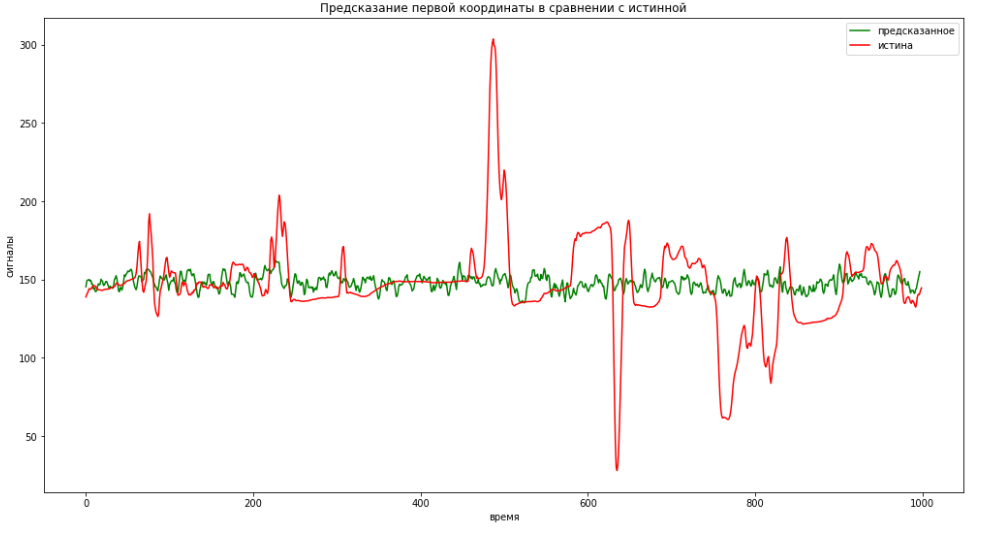
\includegraphics[scale=0.34]{images/5.png}
\end{figure}
Fig. 5. Error analysis depending on the coefficient $\ alpha $ of the SARIMAX and PLS models.
\begin{figure}[H]
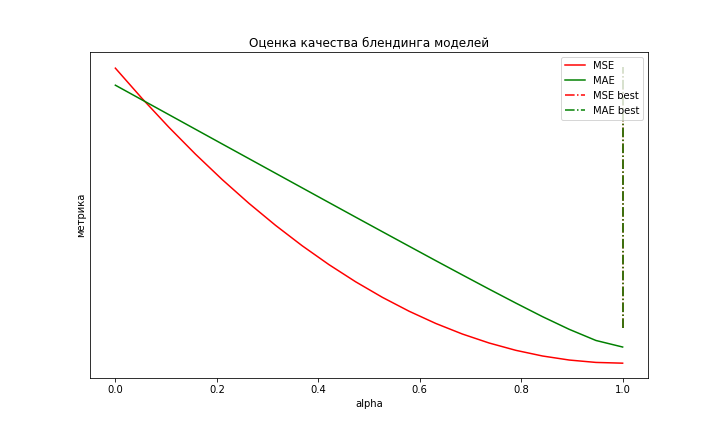
\includegraphics[scale=0.34]{images/6.png}
\end{figure}
Fig. 6. Error analysis depending on the coefficient $\ alpha $ of AR and PLS models.



\section{Error analysis}
Prediction of the time series of the brush coordinates, based on the past points of the trajectory, is considered. It is proposed to compare five models --- $ PLS $ in its pure form, $ SARIMAX $ in its pure form and their mix. And also $ AR $ in its pure form and its coordination with $ PLS $. Comparison is based on metrics $MSE, MAE$.
\begin{figure}[H]
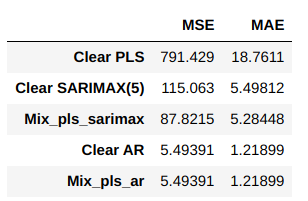
\includegraphics[scale=1]{images/7.png}
\end{figure}
As you can see, agreement the SARIMAX and PLS models gives a better result than each of them separately. The AR model itself is so good that even matching with PLS does not improve prediction, it only spoils it. It can be concluded that simple AR is the best model.
\section{Conclusion}
In the course of the work, various models were proposed and experimentally tested, as well as the agreement of the models.  Based on prediction errors, it is argued that prediction by conventional autoregression gives much less error than other models and their combinations. Also it is shown that agreement models gives better results than each of them separately. Thus, a variation of the problem should be considered when, when testing models, the test series of coordinates of past values is not available, but only the series is available during training. 


\nocite{*}
\bibliographystyle{plain}
\bibliography{references}



\end{document}
